\section{Methodology}
\label{sec:method}

\subsection{Workflow overview}

A bit-accurate reference model is an executable behavior model that is bitwise equivalent to the arithmetic behavior of the corresponding hardware. For each matrix multiplication accelerator (MMA) and each matrix multiplication instruction (MMI), the bit-accurate reference model provides an arithmetic algorithm $f$ such that
\begin{equation}
    f(A,B,C) = \mathrm{MMI}_{\mathrm{MMA}}(A,B,C),
\end{equation}
given any input matrices $A$, $B$, and $C$ with the shape and data type specified by the MMI.

To build this bit-accurate reference model, we adopt a testing-based, non-intrusive approach, treating the hardware behavior as a black box. Specifically, for each generation of Tensor Cores and Matrix Cores, we examine each MMI, and build an arithmetic algorithm $f$ for the MMI following the workflow shown below.

\begin{enumerate}
    \item First, we construct specially crafted inputs to test the MMI, and detect the characteristics of the MMI according to its output on the MMA. The characteristics include summation order, accumulation precision, rounding modes, special value handling rules, etc.
    \item Based on the detected characteristics, we construct an algorithm to compute Equation \ref{eq:mm}, and implement this algorithm with Python.
    \item Then, we validate the correctness of the algorithm by comparative testing. Given over a million sets of random inputs, if the outputs of our algorithm are bitwise consistent with the outputs of hardware, we stop here and examine the next MMI.
    \item Otherwise, we analyze the differences in the outputs and refine our algorithm accordingly to fix the mismatch. The test and refinement are repeated until the validation succeeds.
\end{enumerate}

In the remainder of this section, we first show that modeling the matrix multiply-add operation of MMIs can be simplified to modeling the dot-add operation. Then, we introduce the main characteristics we test and how we design special inputs for them.

\subsection{Problem simplification}

We first check whether each element of the output matrix $D$ is computed in the same way---that is, whether the dot-add computation 
\begin{equation}
\label{eq:dij}
    d_{ij} = c_{ij}+\sum_{k=0}^{K-1} a_{ik}b_{kj}
\end{equation}
depends on the indices $i$ and $j$. To test this, we first set $i=0$ and $j=0$ and generate random inputs $a_{0k}$, $b_{k0}$, and $c_{00}$ for $k=0,1,...,K-1$. Then, we set $a_{ik}=a_{0k}$, $b_{kj}=b_{0j}$, and $c_{ij}=c_{00}$ for all other $i$ and $j$. By sending the input to the MMA, we see that each element $d_{ij}$ in the output is bitwise identical. We observe such consistent behavior across large-scale random tests. Therefore, each output element in $D$ is computed in the same way.

In the following part of this paper, we simplify the notation of Equation \ref{eq:dij} to
\begin{equation}
\label{eq:d}
\begin{split}
    d &= c + \sum_{k=0}^{K-1}a_{k}b_{k} \\
     &= f(c, a_0, a_1, ..., a_{K-1}, b_0, b_1, ..., b_{K-1}).
\end{split}
\end{equation}
Hence, our goal is reduced to building a $(2K+1)$-input algorithm $f(c, \mathbf{a}, \mathbf{b})$ for the dot-add computation of each MMI.

\subsection{Summation order}

We use specially crafted inputs to detect the summation order in the computation of Equation \ref{eq:d}. The inputs are constructed so that the $K+1$ summands
\begin{equation}
    p_k=\begin{cases}
        a_kb_k &\text{if $0\le k < K$} \\
        c &\text{if $k=K$}
    \end{cases}
\end{equation}
consist of a very large power of two $X$, its negation $-X$, and $K-1$ numbers with the same value $y$ that is a very small power of two. When sending such input to the MMA, the hardware output divided by $y$ represents the number of summands summed after the neutralization of $p_i+p_j=0$ where $p_i=X$ and $p_j=-X$, so we can determine the priority of the summation operation between $p_i$ and $p_j$. We run this numerical experiment with $X$ and $-X$ at different locations, so we can construct the summation tree based on the priority information. We construct the summation tree by leveraging the tree construction algorithms in \cite{xie_revealing_2025}.

As a result, we can generate a summation tree that represents the summation order. For example, Figure \ref{fig:tree} shows four typical summation trees that we construct for MMIs on all generations of Tensor Cores and Matrix Cores. 

\begin{figure}[ht]
\begin{subfigure}[b]{0.4\linewidth}
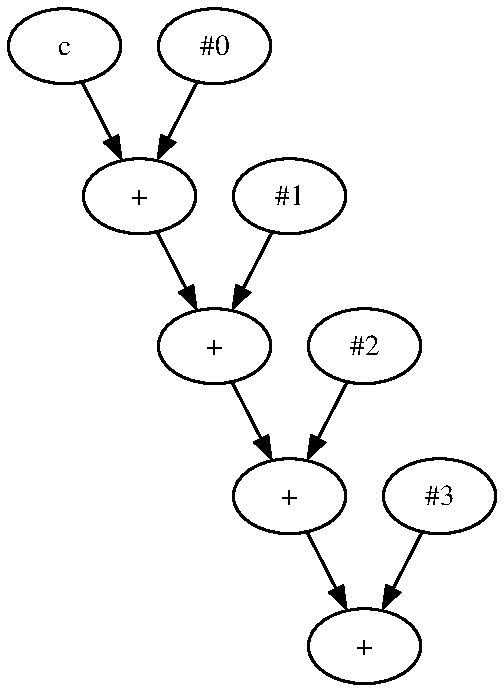
\includegraphics[width=0.8\linewidth]{figures/sequential.pdf}
\caption{Sequential summation.}
\end{subfigure}
\begin{subfigure}[b]{0.6\linewidth}
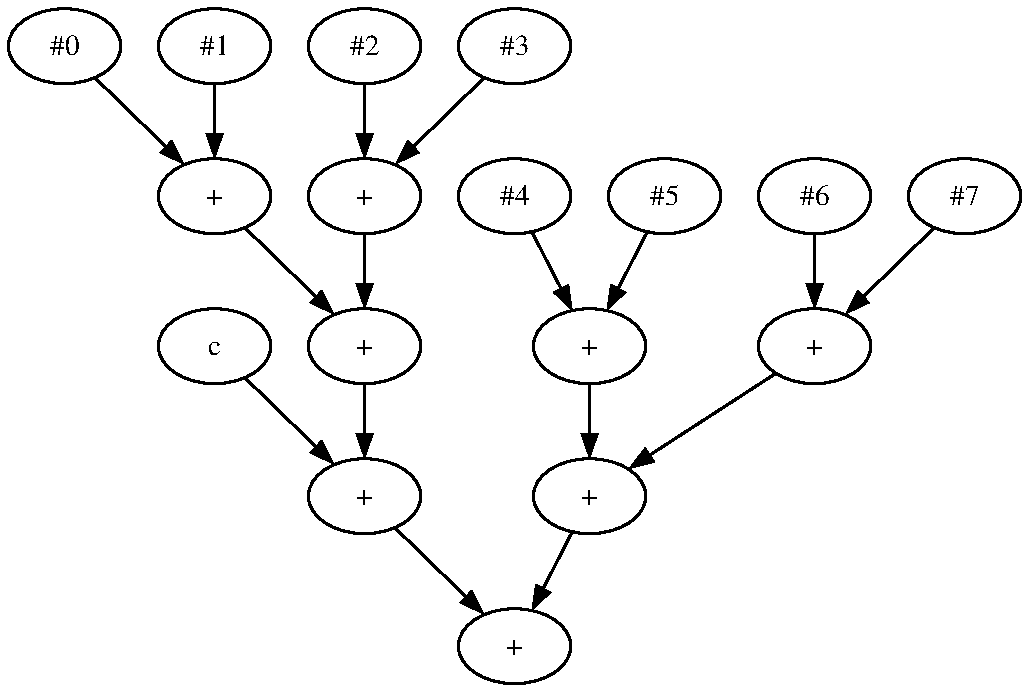
\includegraphics[width=1\linewidth]{figures/pairwise.pdf}
\caption{Group pairwise summation.}
\end{subfigure}
\begin{subfigure}[b]{0.4\linewidth}
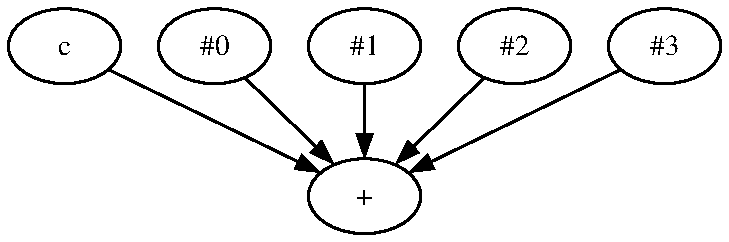
\includegraphics[width=1\linewidth]{figures/fused.pdf}
\caption{Fused summation.}
\end{subfigure}
\begin{subfigure}[b]{0.6\linewidth}
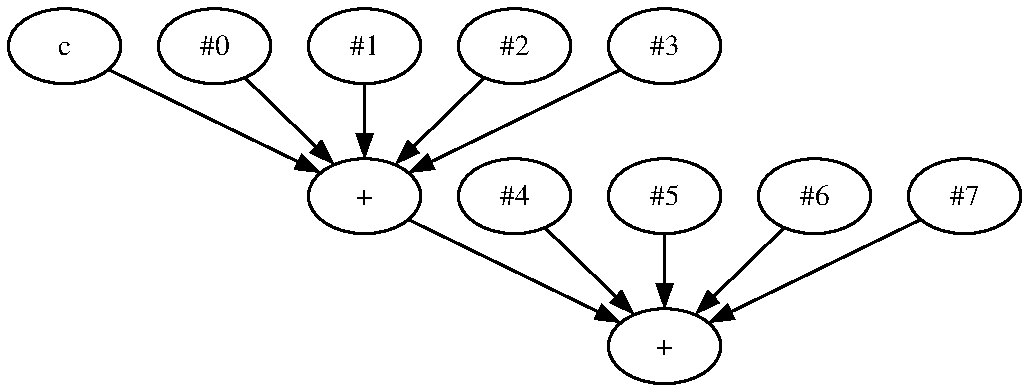
\includegraphics[width=1\linewidth]{figures/chain_of_fused.pdf}
\caption{Chain of fused summations.}
\end{subfigure}
\caption{Four typical summation orders on Tensor Cores and Matrix Cores. \#$i$ represents the product $a_ib_i$.}
\label{fig:tree}
\end{figure}

The first two summation trees are binary trees, representing that the summation is composed of binary addition operations with different orders. Figure \ref{fig:tree}(a) shows the summation tree of the DMMA.884 instruction on the Ampere architecture, indicating the sequential summation order. Figure \ref{fig:tree}(b) shows the summation tree of the v\_mfma\_f32\_32x32x8\_f16 instruction on the CDNA2 architecture, indicating the pairwise summation order within groups of four summands and the sequential summation order among $c$ and the group sums. 

The last two summation trees are multiway trees. A $t$-ary tree represents that the summation is based on $t$-term fused summation, which means that the $t$ terms are summed before the intermediate summation result is normalized to the floating-point number. Figure \ref{fig:tree}(c) shows the summation tree of the HMMA.1684.F32.TF32 instruction on the Ampere architecture, indicating that the 5-term fused summation is used. Figure \ref{fig:tree}(d) shows the summation tree of the HMMA.1688.F32.TF32 instruction on the Ampere architecture, indicating that two five-term fused summations are used iteratively.

\subsection{Accumulation precision}

We use specially crafted inputs to detect the precision in the summation of Equation \ref{eq:d}. For each summation based on binary addition operations, we use $1.0 + \epsilon$ to test its precision. Specifically, for the summation of $p_i$ and $p_j$, we first set $p_i=1.0$ and $p_j=\epsilon=1.0$, and set other summands to zero. Next, we repeatedly halve $\epsilon$ until the hardware output satisfies $d\neq 1.0+\epsilon$. Then, we conclude that the accumulation precision of $p_j$ in this operation is $1-\log_2 \epsilon$ bits after the radix point. We can determine the precision of all summands in all addition operations by running this numerical experiment with different $i$ and $j$ indices.

For each $t$-term fused summation, we use $-1.0+1.0+\epsilon$ to test the precision of the operation. Similarly, for the summation operation including $p_i$, $p_j$, and $p_k$, we first set $p_i=-1.0$, $p_j=1.0$, and $p_k=\epsilon=1.0$, and set other summands to zero. Next, we continuously halve $\epsilon$ until the hardware output $d\neq \epsilon$. Then, we conclude that the precision of $p_k$ is $1-\log_2 \epsilon$ bits after the radix point. We can determine the precision of all summands in all summation operations by running this numerical experiment with different $i$, $j$, and $k$ indices.

\subsection{Rounding mode}

After detecting the accumulation precision, we analyze the rounding mode for each summation operation by specially crafted inputs. We first set the unit in the last place $u=2\epsilon$. Then, we construct the input to make the unrounded sum equal to $1.0+0.75u$, $1.0+0.25u$, $-1.0-0.75u$, and $-1.0-0.25u$. According to the rounded results, we refer to Table \ref{tab:rounding} and identify the rounding mode, which can be rounding up (RU), rounding down (RD), rounding to zero (RZ), rounding away from zero (RA), or rounding to nearest (RN).

\begin{table}[ht]
\caption{Rounding mode detection according the rounding results of four inputs.}
\label{tab:rounding}
\centering
\begin{tabular}{|l|l|l|l|l|}
\hline
Input & $1+0.75u$ & $1+0.25u$ & $-1-0.75u$ & $-1-0.25u$ \\ \hline
RU & $1+u$ & $1+u$ & $-1$ & $-1$ \\ \hline
RD & $1$ & $1$ & $-1-u$ & $-1-u$ \\ \hline
RZ & $1$ & $1$ & $-1$ & $-1$ \\ \hline
RA & $1+u$ & $1+u$ & $-1-u$ & $-1-u$ \\ \hline
RN & $1+u$ & $1$ & $-1-u$ & $-1$ \\ \hline
\end{tabular}
\end{table}

If the rounding mode belongs to RN, we further test $1.0+0.5u$, $1.0+1.5u$, $-1.0-0.5u$, and $-1.0-1.5u$. According to the rounded results, we refer to Table \ref{tab:rn} and identify the tie-breaking rule of RN, which can be rounding ties up (RNU), rounding ties down (RND), rounding ties to zero (RNZ), rounding ties away from zero (RNA), rounding ties to even (RNE), or rounding ties to odd (RNO).

\begin{table}[ht]
\caption{Tie-breaking rule detection for rounding-to-nearest modes according the rounding results of four inputs.}
\label{tab:rn}
\centering
\begin{tabular}{|l|l|l|l|l|}
\hline
Input & $1+0.5u$ & $1+1.5u$ & $-1-0.5u$ & $-1-1.5u$ \\ \hline
RNU & $1+u$ & $1+u$ & $-1$ & $-1-u$ \\ \hline
RND & $1$ & $1+u$ & $-1-u$ & $-1-2u$ \\ \hline
RNZ & $1$ & $1+u$ & $-1$ & $-1-u$ \\ \hline
RNA & $1+u$ & $1+2u$ & $-1-u$ & $-1-2u$ \\ \hline
RNE & $1$ & $1+2u$ & $-1$ & $-1-2u$ \\ \hline
RNO & $1+u$ & $1+u$ & $-1-u$ & $-1-u$ \\ \hline
\end{tabular}
\end{table}

\subsection{Special value handling}

Subnormal numbers, negative zero, infinity, and NaNs are special values in floating-point arithmetic. We construct inputs in edge conditions to detect the special value handling rules of the MMI.

For subnormal numbers, we first set $c$ to $0.5\epsilon$ (where $\epsilon$ is the smallest positive normal number) and set other inputs to zero. If the hardware output equals zero, it indicates that the subnormal input of $c$ is flushed to zero. Similarly, we set an input $a_k$ (or $b_k$) to $0.5\epsilon$, set the corresponding $b_k$ (or $a_k$) to one, and set other inputs to zero. If the hardware output equals zero, it indicates that the subnormal input of $a_k$ (or $b_k$) is flushed to zero. Next, we detect whether subnormal values will be flushed after multiplication by setting an input $a_k=0.5$, setting its corresponding $b_k=\epsilon$, and setting other inputs to zero. Finally, we detect whether subnormal values will be flushed after addition by setting a summand $p_i=1.5\epsilon$, setting another summand $p_j=-\epsilon$, and setting other inputs to zero.

For negative zeros, we detect whether a negative zero can be generated by setting the inputs to $-0.0+\sum_{k=0}^{K-1}(+0.0)\times(-0.0)$. Whether the hardware output equals $-0.0$ indicates whether the negative zero can be generated.

For infinity, we detect whether multiplication can overflow by setting $a_k=2.0$ for some $k$, setting $b_k=2^E$, $c=-2^E$, and setting other inputs to zero, where $E$ is the maximum exponent of the input floating-point format. We also detect whether intermediate summation can overflow by testing $2^E+2^E-2^E$. Then, we detect the rules for overflows by testing the edge conditions $(2-u)\times2^E+0.75u\times2^E$, $(2-u)\times2^E+0.5u\times2^E$, $(2-u)\times2^E+0.25u\times2^E$, $(-2+u)\times2^E-0.75u\times2^E$, $(-2+u)\times2^E-0.5u\times2^E$, and $(-2+u)\times2^E-0.25u\times2^E$.

For NaNs, we set $p_k=0.0\times\infty$ for some $k$, and set other inputs to zero; then we set $p_i=-\infty$ and $p_j=+\infty$ for some $i$ and $j$, and set other inputs to zero. We find that NaNs can be generated in both cases for all the tested MMAs.